\documentclass[11pt,letterpaper]{article}

\usepackage{parskip}
\usepackage{graphicx}
\usepackage{float}
\usepackage[margin=1in]{geometry}

\title{\textsc{LOSeR:} Linked Offset Storage/Retrieval \\ \large \textit{An Experimental Data Calibration Database System}}
\author{Mark D. Hare \\ \texttt{markhare@buffalo.edu}}

\newcommand{\loser}{\textsc{LOSeR\ }}


\begin{document}
\maketitle

\section{Purpose}
The Linked Offset Storage/Retrieval system (affectionately referred to as ``\loser'') is a data acquisition workflow with an associated software implementation. \loser is a database system that allows experimental calibration data to be collected, stored, and linked to associated experimental trials. This allows the researcher to avoid the tedium of recalibration and the chaos of calibration storage and documentation. The \loser process integrates easily with existing data acquisition workflows and reduces the danger of lost or misinterpreted experimental data.

\section{Architecture}

\begin{figure}[h]
\centering
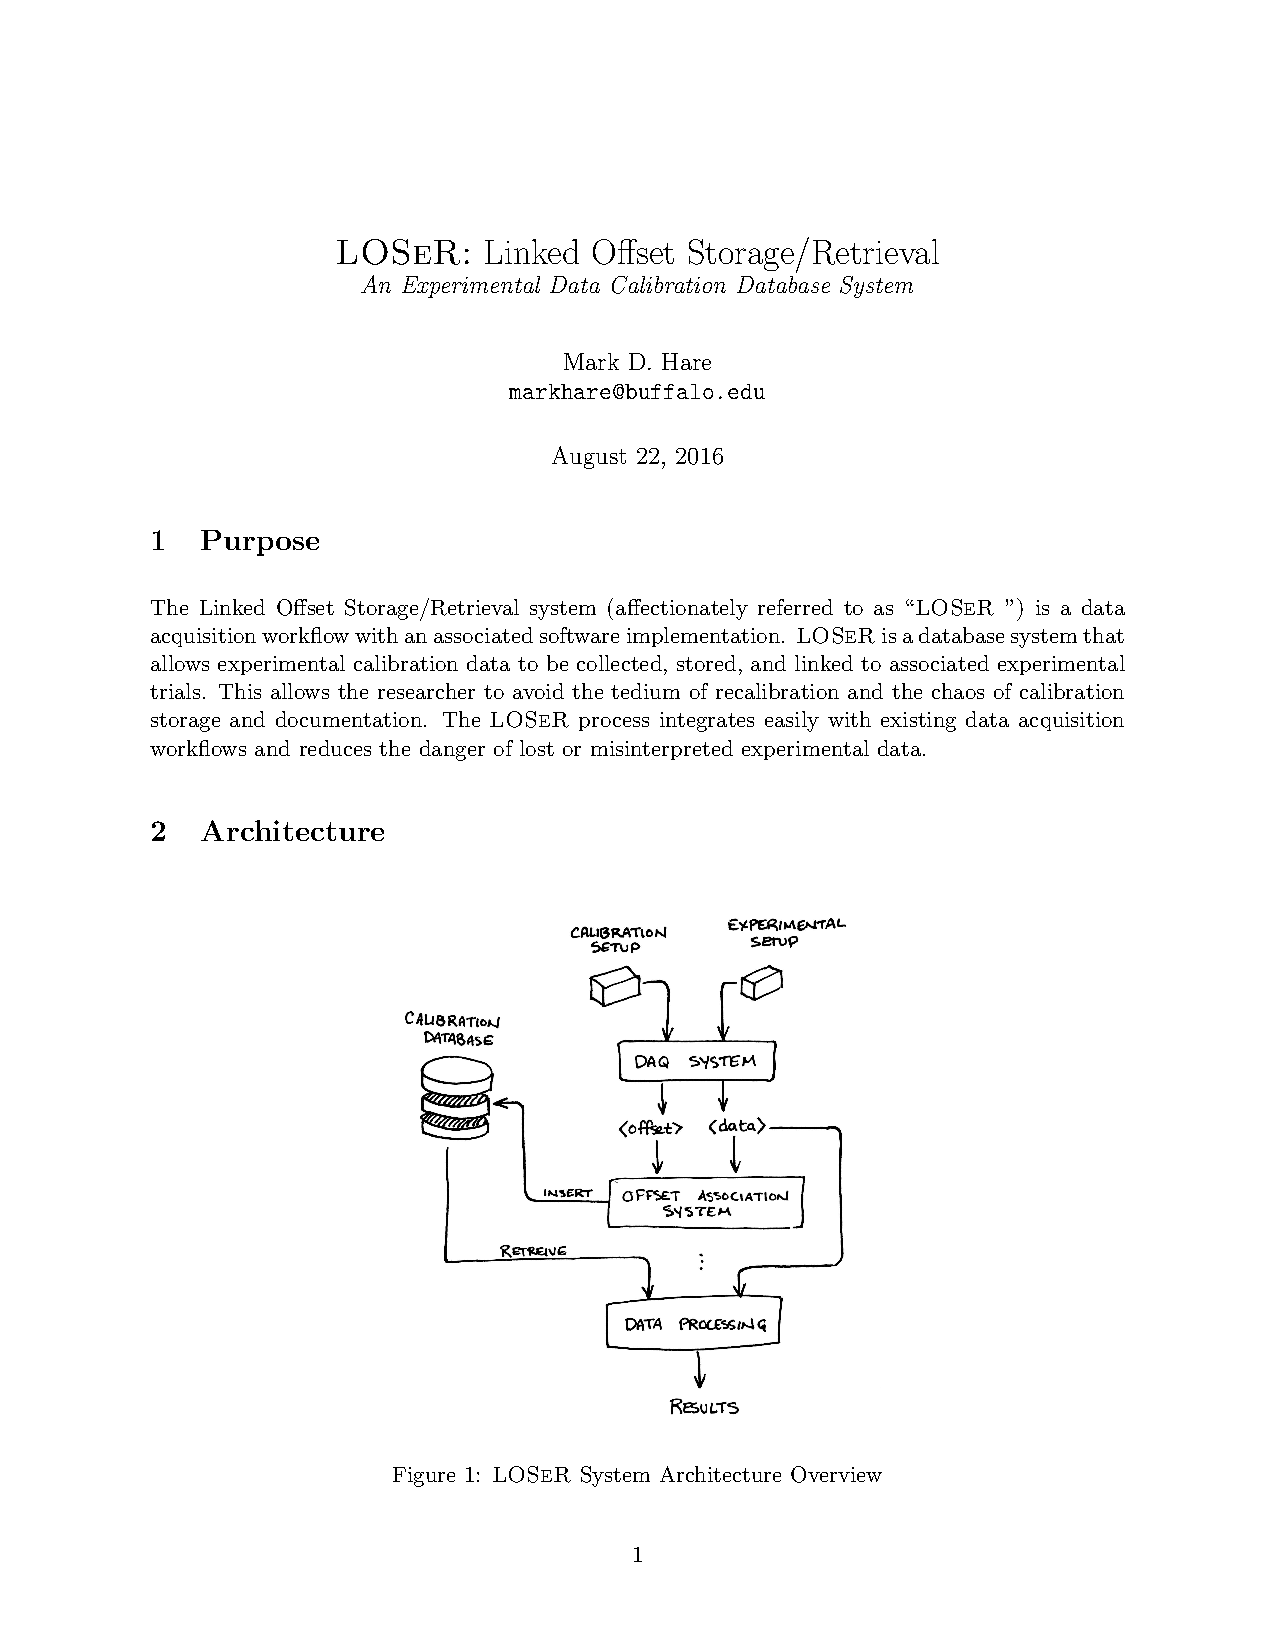
\includegraphics[width=0.5\textwidth]{loser}
\caption{\loser System Architecture Overview}
\label{fig:arch}
\end{figure}

Steps in \loser workflow (see figure \ref{fig:arch} for diagram of system architecture):
\begin{enumerate}
\item Set up experiment in zeroed or calibration state and acquire calibration data
\item For each test in the group of test for which this calibration is valid:
\begin{enumerate}
\item Perform test and acquire data
\item Associate calibration with test using Offset Association System
\end{enumerate}
\item Process data for each test as necessary, retrieving linked calibrations from database
\end{enumerate}

\section{Implementation}

The working implementation of \loser will use a data acquisition system based on National Instruments' LabVIEW, association and processing scripts written in \textsc{matlab}, and an SQLite database system for offset storage. The \textsc{matlab}/SQLite connector is a \textsc{matlab} extension written in C by Robin Martinjak, available at \texttt{https://github.com/rmartinjak/mex-sqlite3} under an MIT license.

\end{document}
